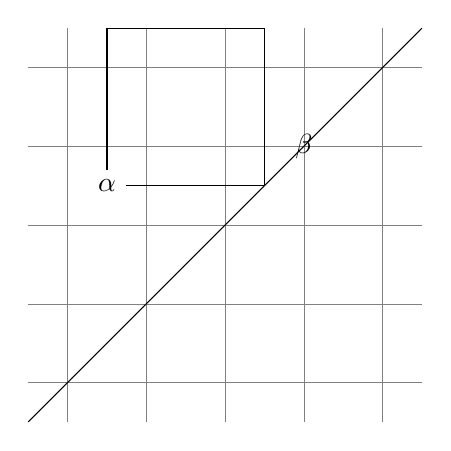
\begin{tikzpicture}    %[nomestile/.style={opzioni}]
    %linee guida
    \draw [help lines] (-2.5,-2.5) grid (2.5,2.5);

    % Cambio posizione corrente
    \path (1,0);
    % \draw[opzioni] (coordinate pt iniziale)--(coordinate pt finale);
    \draw (-2.5,-2.5)--(2.5,2.5);

    %\node[opzioni] (label) at (coordinata pt) {testo}; 
    \node (origine) at(-1.5,0.5) {$\alpha$};
    \node at (1,1) {$\beta$};

    \draw (origine) -| ++(2,2) -| (origine);
    

\end{tikzpicture}
